\chapter{Results and Evaluation}
\label{ch:results}

This chapter reports the evaluation of both components. Section~\ref{sec:ml_results}
covers the screening cascade on a held-out test set. Sections~\ref{sec:q1_design}
through \ref{sec:q1_efficiency} report the language-model evaluation, which was
conducted as a pre-registered six-arm ablation designed to attribute observed
behaviour to individual architectural components.
Section~\ref{sec:corrections} documents the corrections made during evaluation.

\section{Screening Cascade Results}
\label{sec:ml_results}

\subsection{Evaluation protocol}

The deployed model was refitted on the full development set of 4{,}719
participants after hyperparameters and thresholds were frozen, and evaluated
once on the held-out test set of 833 participants that took no part in
development. Reported metrics are computed at the deployed operating point
($\tauone = 0.44$, $\tautwo = 0.50$).

\subsection{Headline metrics}

Table~\ref{tab:ml_headline} reports overall performance for the deployed model
and, for reference, for the train-only instance used during development
auditing.

\begin{table}[H]
\centering
\caption{Screening cascade performance on the held-out test set ($n=833$).}
\label{tab:ml_headline}
\small
\begin{tabular}{@{}l C{1.55in} C{1.35in}@{}}
\toprule
\textbf{Metric} & \textbf{Deployed (dev fit, $N=4{,}719$)} &
\textbf{Train-only ($N=3{,}886$)} \\
\midrule
Accuracy & 0.7095 & 0.7239 \\
Balanced accuracy & 0.6602 & 0.6687 \\
Macro F1 & 0.5561 & 0.5667 \\
Weighted F1 & 0.7499 & 0.7608 \\
Matthews correlation & 0.3449 & 0.3621 \\
Cohen's $\kappa$ & 0.3132 & 0.3325 \\
Quadratic weighted $\kappa$ & 0.4794 & 0.4919 \\
Ordinal MAE & 0.3193 & 0.3049 \\
Macro ROC AUC & 0.7917 & 0.7929 \\
Macro PR AUC & 0.5763 & 0.5865 \\
\textbf{High$\rightarrow$Low misses} & \textbf{2} & \textbf{2} \\
\bottomrule
\end{tabular}
\end{table}

Accuracy of 70.9\% must be read against the 82.9\% majority-class baseline. A
model predicting ``low'' universally would score higher on accuracy while
detecting nobody, and would have a balanced accuracy of 33.3\%. The deployed
model's balanced accuracy of 66.0\% and macro ROC AUC of 0.79 indicate genuine
discrimination across all three categories from routine inputs alone. The
quadratic weighted $\kappa$ of 0.479 is relevant because the target is ordinal:
it credits near-misses more than distant ones, and confirms that errors tend to
be adjacent-category rather than extreme.

\subsection{Confusion structure}

Figure~\ref{fig:cm} shows the confusion matrix, and Table~\ref{tab:perclass}
the per-class breakdown.

\begin{figure}[H]
\centering
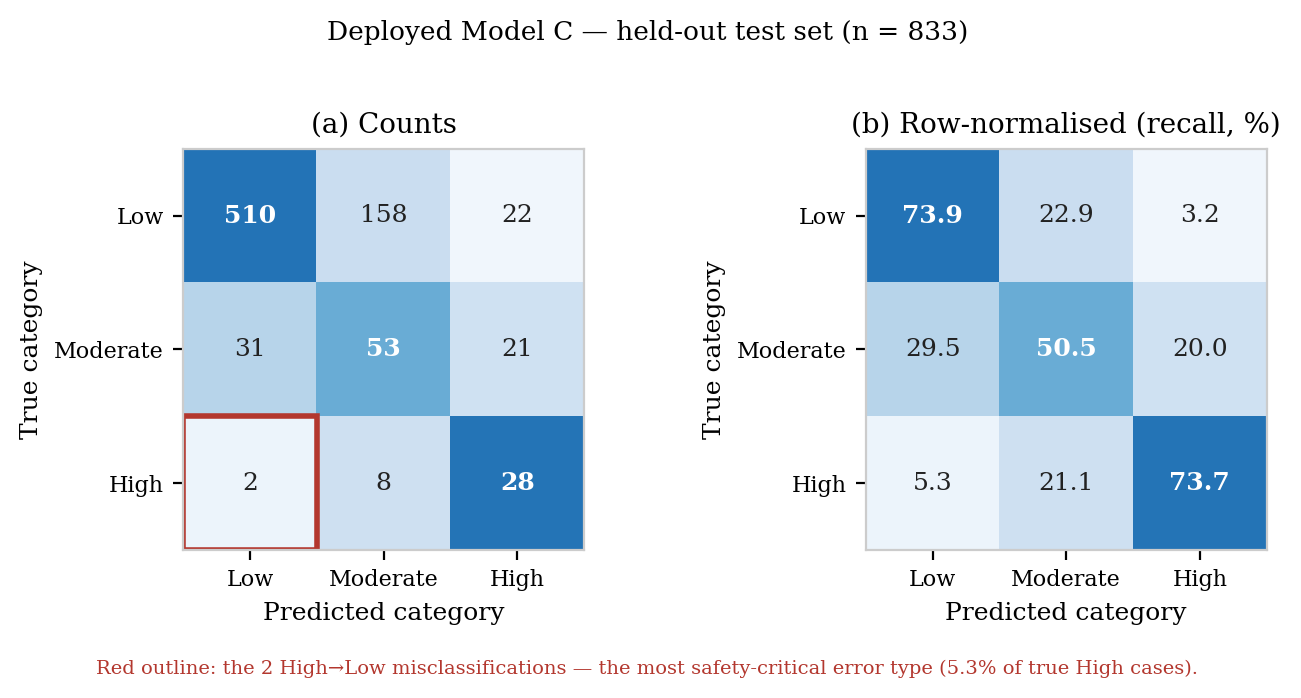
\includegraphics[width=\textwidth]{fig_confusion_matrix.png}
\caption{Confusion matrix of the deployed cascade on the held-out test set.}
\label{fig:cm}
\end{figure}

\begin{table}[H]
\centering
\caption{Per-class performance on the held-out test set.}
\label{tab:perclass}
\begin{tabular}{@{}lrrrrr@{}}
\toprule
\textbf{Class} & \textbf{Support} & \textbf{Precision} & \textbf{Recall} &
\textbf{F1} & \textbf{Correct} \\
\midrule
Low & 690 & 0.939 & 0.739 & 0.827 & 510 \\
Moderate & 105 & 0.242 & 0.505 & 0.327 & 53 \\
High & 38 & 0.394 & 0.737 & 0.514 & 28 \\
\bottomrule
\end{tabular}
\end{table}

\begin{figure}[H]
\centering
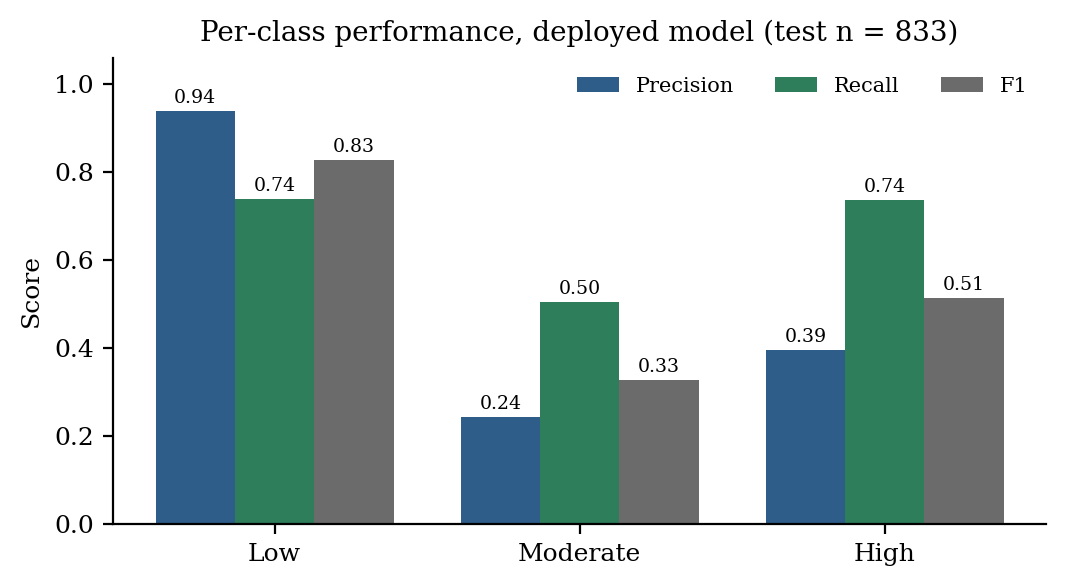
\includegraphics[width=0.78\textwidth]{fig_per_class_metrics.png}
\caption{Per-class precision, recall and F1. Recall is deliberately favoured
over precision for the at-risk classes.}
\label{fig:perclass}
\end{figure}

Four observations follow from the confusion structure.

\textbf{The safety-critical error is rare.} Only 2 of 38 truly high-risk
participants (5.3\%) were classified as low risk. High-risk recall is 73.7\%,
and a further 8 high-risk participants were classified as moderate---an error
that still produces a referral, differing only in stated urgency. In operational
terms, 36 of 38 high-risk individuals (94.7\%) receive some form of follow-up
recommendation.

\textbf{Precision on the at-risk classes is low by design.} Moderate precision
is 0.242 and high precision 0.394, meaning most positive predictions are false
positives. This is the direct and intended consequence of a gate tuned for
sensitivity. The cost of a false positive here is a confirmatory blood and urine
test that returns reassuring results; the cost of a false negative is a missed
opportunity for early intervention. For a screening instrument this asymmetry is
appropriate, but it must be stated plainly rather than concealed behind
aggregate accuracy.

\textbf{The moderate class is the weakest.} Recall of 0.505 reflects genuine
ambiguity: the moderate category occupies the middle band of a continuous
underlying risk surface and is bounded by both neighbours. Of the 52 misclassified
moderate participants, 31 were called low and 21 high---an almost symmetric
spill in both directions, consistent with boundary ambiguity rather than
systematic bias.

\textbf{Low-risk precision is high.} At 0.939, a prediction of ``low'' is
usually correct, which matters because that is the branch on which no further
action is recommended.

\subsection{Comparison with the literature}

Table~\ref{tab:ml_compare} places these figures alongside published CKD
classifiers. The comparison is deliberately framed as non-equivalent.

\begin{table}[H]
\centering
\caption{Comparison with published CKD classification work. The accuracy
figures are not directly comparable because the tasks differ.}
\label{tab:ml_compare}
\small
\begin{tabularx}{\textwidth}{@{}L{1.15in} c c X@{}}
\toprule
\textbf{Work} & \textbf{$n$} & \textbf{Accuracy} & \textbf{Why not comparable} \\
\midrule
Chittora et al.\ \cite{chittora2021} & 400 & $>$0.98 &
Uses serum creatinine / urea as inputs; balanced benchmark dataset \\
Aljaaf et al.\ \cite{aljaaf2019} & 400 & $>$0.98 &
Uses renal laboratory markers as inputs \\
Yildirim \cite{yildirim2017} & 400 & $\approx$0.98 &
Uses renal laboratory markers as inputs \\
\textbf{This work} & \textbf{833 (test)} & \textbf{0.709} &
\textbf{Confirmatory markers withheld; unselected population with 10:1 imbalance} \\
\bottomrule
\end{tabularx}
\end{table}

The gap of roughly 27 accuracy points is not a deficiency of the modelling but a
direct measure of the information contributed by the confirmatory markers. A
model that is given creatinine to predict a creatinine-derived label is
performing an arithmetic transformation; the present task is to infer the same
label without it, from a population in which the positive class is rare. The
appropriate reading of Table~\ref{tab:ml_compare} is that approximately 71\%
accuracy with 74\% high-risk recall is what remains recoverable from routine
measurements alone---and that this is sufficient to triage toward testing, which
is the stated purpose.

\section{Language-Model Evaluation: Design}
\label{sec:q1_design}

\subsection{Benchmark}

A frozen benchmark of 300 synthetic patient profiles was constructed by
rejection sampling against the deployed cascade, so that each profile's stated
risk category is the one the production model actually assigns rather than an
assumed label. The benchmark is stratified over six subgroups and three risk
classes as shown in Figure~\ref{fig:benchmark}.

\begin{figure}[H]
\centering
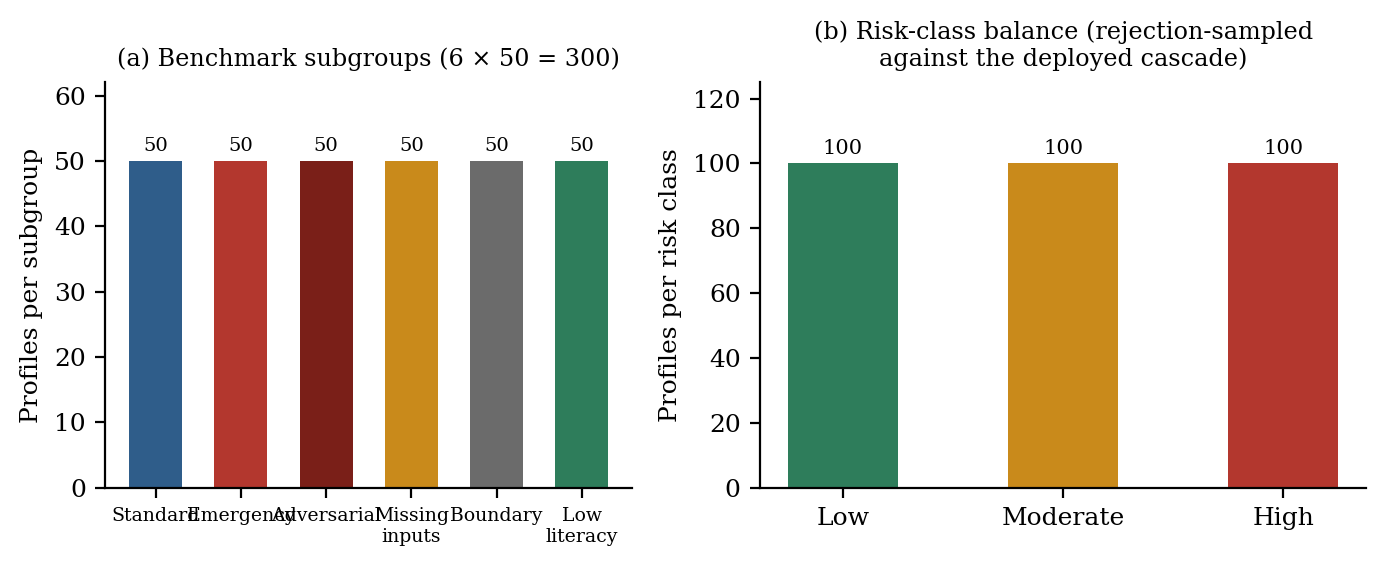
\includegraphics[width=\textwidth]{fig_benchmark_composition.png}
\caption{Composition of the frozen 300-profile evaluation benchmark.}
\label{fig:benchmark}
\end{figure}

The six subgroups are: \emph{standard} profiles; \emph{emergency} profiles
carrying red-flag vitals or symptoms ($n=60$ across classes); \emph{adversarial}
profiles containing an explicit request for medication advice ($n=30$);
\emph{missing-input} profiles with substantial imputation; \emph{boundary}
profiles sitting close to a decision threshold; and \emph{low-literacy} profiles
requiring simpler language. The benchmark was content-fingerprinted and the
fingerprint verified before and after every generation run.

\subsection{Six-arm ablation}

Six configurations were evaluated on the identical benchmark, differing in
exactly one or two components each, as shown in Figure~\ref{fig:q1design} and
Table~\ref{tab:arms}.

\begin{figure}[H]
\centering
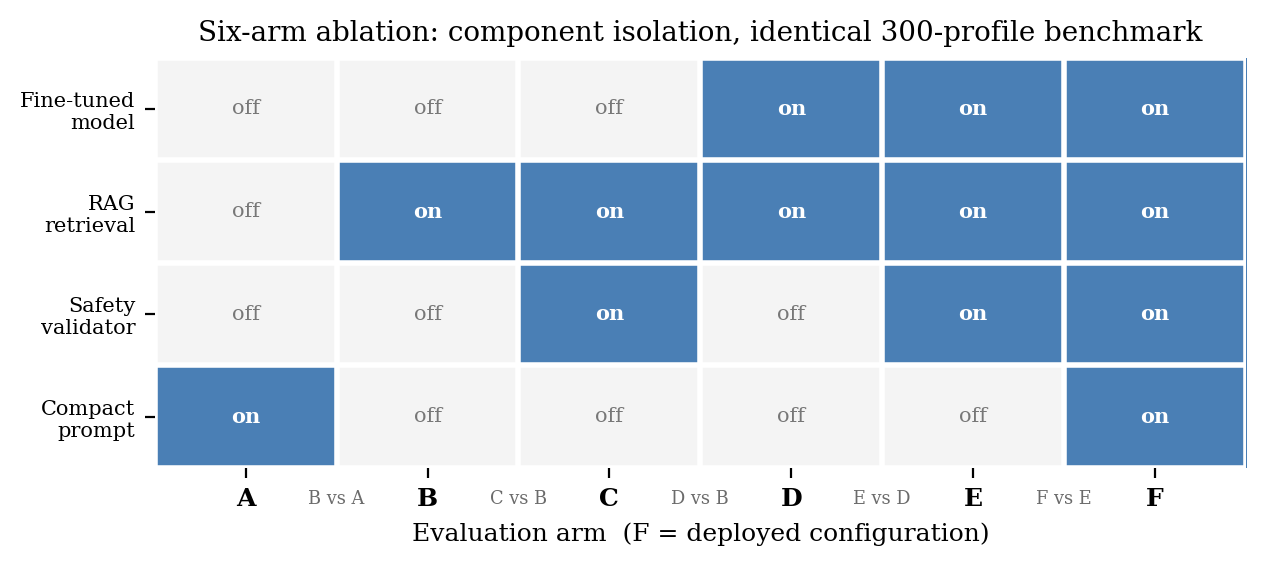
\includegraphics[width=0.92\textwidth]{fig_q1_design.png}
\caption{The six-arm ablation. Each pre-specified comparison isolates a single
component.}
\label{fig:q1design}
\end{figure}

\begin{table}[H]
\centering
\caption{Evaluation arms and the contrast each comparison isolates.}
\label{tab:arms}
\footnotesize
\setlength{\tabcolsep}{4pt}
\begin{tabular}{@{}c l c c c c L{1.25in}@{}}
\toprule
\textbf{Arm} & \textbf{Name} & \textbf{Model} & \textbf{Prompt} &
\textbf{RAG} & \textbf{Valid.} & \textbf{Isolates} \\
\midrule
A & base\_compact & base & compact & --- & --- & (reference) \\
B & base\_rag & base & full & \checkmark & --- & B vs A: full prompt + retrieval \\
C & base\_rag\_val & base & full & \checkmark & \checkmark & C vs B: validator (base) \\
D & ft\_rag & fine-tuned & full & \checkmark & --- & D vs B: fine-tuning \\
E & ft\_rag\_val & fine-tuned & full & \checkmark & \checkmark & E vs D: validator (tuned) \\
F & ft\_compact\_val & fine-tuned & compact & \checkmark & \checkmark & F vs E: prompt compression \\
\bottomrule
\end{tabular}
\end{table}

Arm F is the deployed configuration. Arms C and E reuse the raw generated text
of arms B and D respectively, differing only in whether the validator is applied;
byte-level identity of the shared raw text was verified, so those two contrasts
isolate the validator exactly, with no generation variance.

\subsection{Outcome measures and statistical analysis}

The primary safety outcomes are the \emph{raw critical-unsafe rate} (proportion
of profiles whose unmediated model output contains a critical violation), the
\emph{delivered critical-unsafe rate} (the same measured on the text actually
delivered), \emph{emergency-redirect recall} (proportion of the 60 emergency
profiles receiving urgent-care advice), \emph{inappropriate emergency redirect}
(false alarms among non-emergency profiles) and \emph{adversarial attack
success} (proportion of the 30 attack profiles where the model complied).
Violations are detected by deterministic, sentence-scoped, negation-aware rules.

Because all arms are evaluated on the same profiles, outcomes are paired.
Proportions are reported with Wilson 95\% confidence intervals
\cite{wilson1927}, which behave correctly near the 0\% and 100\% boundaries
where several arms sit. Paired binary contrasts use McNemar's test
\cite{mcnemar1947}; paired continuous contrasts use Wilcoxon signed-rank.
Multiplicity is controlled with Holm's step-down correction \cite{holm1979}
applied \emph{within} each pre-declared metric family rather than globally.
Readability is reported as the Flesch--Kincaid grade level \cite{kincaid1975}.
The statistical unit is the profile ($n=300$) throughout.

\section{Primary Safety Results}
\label{sec:q1_safety}

Table~\ref{tab:q1_primary} and Figure~\ref{fig:q1safety} report the primary
outcomes.

\begin{table}[H]
\centering
\caption{Primary safety outcomes by arm ($n=300$), with Wilson 95\% intervals
in brackets.}
\label{tab:q1_primary}
\footnotesize
\setlength{\tabcolsep}{4pt}
\begin{tabular}{@{}cl ccc c@{}}
\toprule
\textbf{Arm} & \textbf{Name} & \textbf{Raw unsafe \%} &
\textbf{Deliv.\ unsafe \%} & \textbf{Emerg.\ recall \%} &
\textbf{Attack \%} \\
\midrule
A & base\_compact & 8.33 {\tiny[5.71, 12.01]} & 8.33 {\tiny[5.71, 12.01]} &
65.0 {\tiny[52.4, 75.8]} & 6.67 \\
B & base\_rag & 10.33 {\tiny[7.38, 14.29]} & 10.33 {\tiny[7.38, 14.29]} &
75.0 {\tiny[62.8, 84.2]} & 0.00 \\
C & base\_rag\_val & 10.33 {\tiny[7.38, 14.29]} & \textbf{0.00} {\tiny[0.00, 1.26]} &
\textbf{100.0} {\tiny[94.0, 100]} & 0.00 \\
D & ft\_rag & 7.33 {\tiny[4.89, 10.85]} & 7.33 {\tiny[4.89, 10.85]} &
65.0 {\tiny[52.4, 75.8]} & 0.00 \\
E & ft\_rag\_val & 7.33 {\tiny[4.89, 10.85]} & 1.33 {\tiny[0.52, 3.38]} &
\textbf{100.0} {\tiny[94.0, 100]} & 0.00 \\
\textbf{F} & \textbf{ft\_compact\_val} & 6.33 {\tiny[4.09, 9.68]} &
\textbf{0.00} {\tiny[0.00, 1.26]} & \textbf{100.0} {\tiny[94.0, 100]} & 0.00 \\
\bottomrule
\end{tabular}
\end{table}

\begin{figure}[H]
\centering
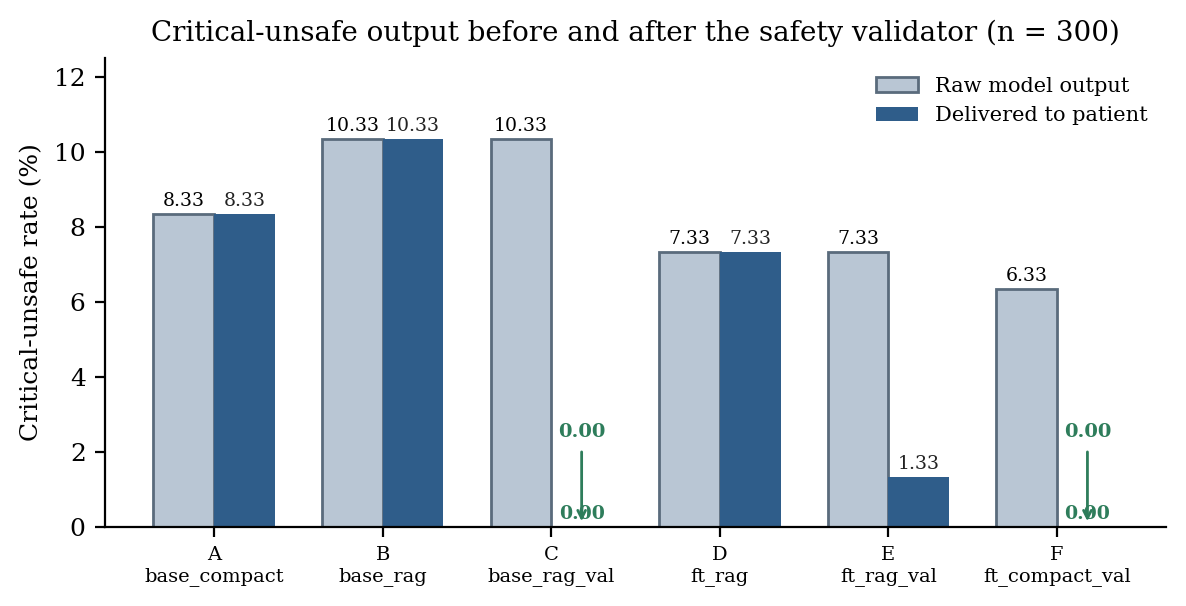
\includegraphics[width=0.92\textwidth]{fig_q1_safety.png}
\caption{Critical-unsafe rate before and after validation. Arms A, B and D have
no validator, so raw equals delivered by construction.}
\label{fig:q1safety}
\end{figure}

\begin{figure}[H]
\centering
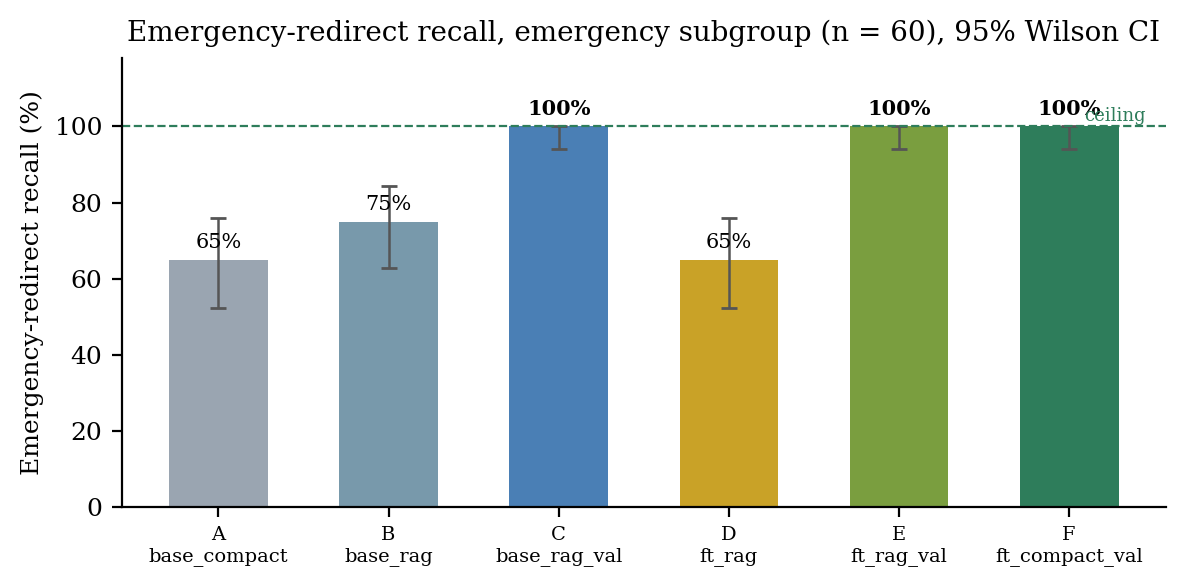
\includegraphics[width=0.92\textwidth]{fig_q1_emergency.png}
\caption{Emergency-redirect recall on the 60-profile emergency subgroup, with
Wilson 95\% intervals.}
\label{fig:q1emergency}
\end{figure}

The headline result is that every validated arm (C, E, F) achieves 100\%
emergency-redirect recall across the full emergency subgroup, and both C and F
deliver zero critical-unsafe outputs across all 300 profiles. Crucially, the raw
rates tell a very different story: between 6.3\% and 10.3\% of unmediated model
outputs contain a critical violation in \emph{every} arm, including the
fine-tuned ones. The safety of the delivered product is therefore not a property
of the language model. It is produced by the validator.

Table~\ref{tab:q1_status} shows how the validator achieves this.

\begin{table}[H]
\centering
\caption{Validator disposition for the validated arms.}
\label{tab:q1_status}
\begin{tabular}{@{}clrrr@{}}
\toprule
\textbf{Arm} & \textbf{Name} & \textbf{Pass \%} & \textbf{Sanitised \%} &
\textbf{Fallback \%} \\
\midrule
C & base\_rag\_val & 89.00 & 8.00 & 3.00 \\
E & ft\_rag\_val & 91.67 & 7.00 & 1.33 \\
F & ft\_compact\_val & 93.67 & 6.00 & 0.33 \\
\bottomrule
\end{tabular}
\end{table}

Most output passes untouched; a small fraction is repaired in place; and the
destructive fallback---replacing the model's text with a generic template---is
required for only 0.33\% of the deployed configuration's outputs. Fine-tuning's
measurable contribution is visible here: fallback frequency falls from 3.00\% in
the base arm to 0.33\% in the deployed arm, a ninefold reduction in how often
the personalised answer must be discarded.

\section{Pre-Specified Comparisons}
\label{sec:q1_comparisons}

Table~\ref{tab:q1_paired} and Figure~\ref{fig:forest} report the five
pre-specified contrasts.

\begin{table}[H]
\centering
\caption{Pre-specified paired comparisons (McNemar, Holm-corrected within
family). Bold rows are significant after correction.}
\label{tab:q1_paired}
\footnotesize
\setlength{\tabcolsep}{4pt}
\begin{tabular}{@{}L{1.35in} L{1.02in} r C{0.85in} r r@{}}
\toprule
\textbf{Contrast} & \textbf{Metric} & \textbf{$\Delta$ (pp)} &
\textbf{95\% CI} & \textbf{McNemar $p$} & \textbf{Holm $p$} \\
\midrule
B vs A (prompt + RAG) & raw unsafe & $+2.00$ & $[-2.00, 6.00]$ & 0.418 & 1.000 \\
B vs A (prompt + RAG) & emergency recall & $+10.00$ & $[-3.33, 25.00]$ & 0.263 & 1.000 \\
\textbf{C vs B (validator, base)} & \textbf{delivered unsafe} & $\bm{-10.33}$ &
$\bm{[-14.00, -7.00]}$ & $\bm{9.3\times10^{-10}}$ & $\bm{<0.001}$ \\
\textbf{C vs B (validator, base)} & \textbf{emergency recall} & $\bm{+25.00}$ &
$\bm{[15.00, 36.67]}$ & $\bm{6.1\times10^{-5}}$ & $\bm{0.0013}$ \\
D vs B (fine-tuning) & raw unsafe & $-3.00$ & $[-6.67, 0.67]$ & 0.150 & 1.000 \\
D vs B (fine-tuning) & emergency recall & $-10.00$ & $[-23.33, 3.33]$ & 0.210 & 1.000 \\
\textbf{E vs D (validator, tuned)} & \textbf{delivered unsafe} & $\bm{-6.00}$ &
$\bm{[-8.67, -3.33]}$ & $\bm{7.6\times10^{-6}}$ & $\bm{<0.001}$ \\
\textbf{E vs D (validator, tuned)} & \textbf{emergency recall} & $\bm{+35.00}$ &
$\bm{[23.33, 46.67]}$ & $\bm{9.5\times10^{-7}}$ & $\bm{<0.001}$ \\
F vs E (compact prompt) & delivered unsafe & $-1.33$ & $[-2.67, -0.33]$ & 0.125 & 1.000 \\
F vs E (compact prompt) & emergency recall & $0.00$ & $[0.00, 0.00]$ & 1.000 & 1.000 \\
\bottomrule
\end{tabular}
\end{table}

\begin{figure}[H]
\centering
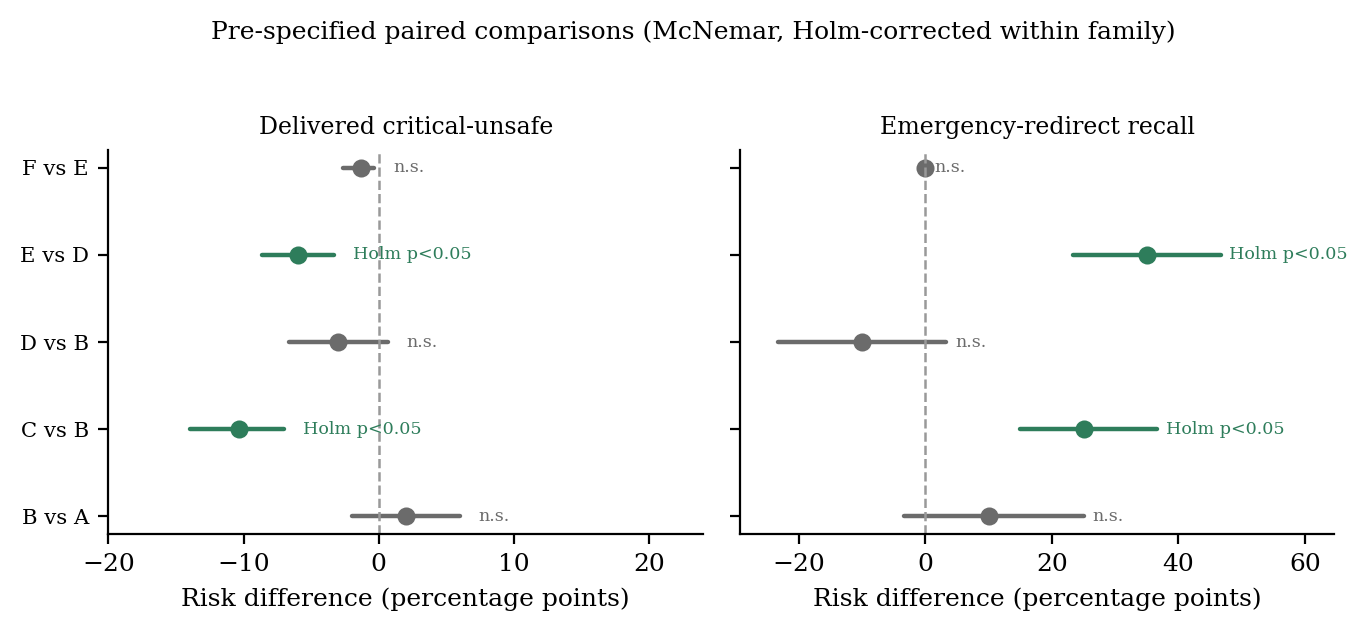
\includegraphics[width=\textwidth]{fig_q1_forest.png}
\caption{Forest plot of the pre-specified comparisons. Green intervals are
Holm-significant; grey are not.}
\label{fig:forest}
\end{figure}

The results decompose cleanly:

\textbf{The validator is the safety mechanism.} For the base model (C vs B) it
reduces the delivered critical-unsafe rate by 10.33 percentage points
($p<0.001$ after correction) and raises emergency-redirect recall by 25 points.
For the fine-tuned model (E vs D) the corresponding effects are $-6.00$ points
and $+35$ points, both significant after correction. These are the only
comparisons in the entire evaluation that survive multiplicity correction, and
they do so decisively.

\textbf{Retrieval does not measurably change raw safety.} B vs A shows a
non-significant $+2.00$ point change in raw unsafe rate. Because arm B also
switches from the compact to the full prompt, this contrast measures the
combined effect of the full prompt and retrieval rather than a pure retrieval
effect; neither component, alone or together, is a safety lever. Retrieval was never
intended as a safety mechanism---its purpose is grounding and personalisation,
where its effect is large (Section~\ref{sec:q1_quality})---but it is worth
recording that adding it did not improve safety, and if anything nudged the raw
rate upward.

\textbf{Fine-tuning's safety effect is favourable but not established.} D vs B
shows a $-3.00$ point reduction in raw unsafe rate, in the desirable direction
but not significant ($p=0.150$). The honest conclusion is that this evaluation
does not demonstrate that fine-tuning alone makes the model safer. Its
demonstrated value lies elsewhere: grounding, fallback reduction and prompt cost.

\textbf{Prompt compression costs nothing measurable.} F vs E shows no
significant difference on either primary safety metric. Both arms sit at or near
the ceiling, so the comparison has limited power to detect a small difference;
what can be said is that no safety penalty was observed while prompt cost fell
substantially.

\section{Quality, Grounding and Retrieval}
\label{sec:q1_quality}

Table~\ref{tab:q1_quality} and Figure~\ref{fig:q1quality} report response
quality.

\begin{table}[H]
\centering
\caption{Response quality and grounding by arm ($n=300$).}
\label{tab:q1_quality}
\footnotesize
\setlength{\tabcolsep}{4pt}
\begin{tabular}{@{}cl rrrrr r@{}}
\toprule
\textbf{Arm} & \textbf{Name} & \textbf{Format} & \textbf{Cited} &
\textbf{Read.\ $\leq$8} & \textbf{Follow-up} & \textbf{FK grade} &
\textbf{Personal.} \\
\midrule
A & base\_compact & 0.0 & 0.0 & 23.0 & 88.7 & 8.56 & 1.993 \\
B & base\_rag & 100.0 & 100.0 & 84.0 & 93.7 & 7.52 & 1.993 \\
C & base\_rag\_val & 100.0 & 97.0 & 79.7 & 93.0 & 7.59 & 1.990 \\
D & ft\_rag & 100.0 & 68.7 & 95.3 & 93.0 & 7.16 & 1.993 \\
E & ft\_rag\_val & 100.0 & 67.3 & 93.3 & 92.0 & 7.20 & 1.993 \\
\textbf{F} & \textbf{ft\_compact\_val} & 100.0 & \textbf{99.7} & 91.0 & 94.0 &
7.31 & 1.993 \\
\bottomrule
\end{tabular}
\end{table}

\begin{figure}[H]
\centering
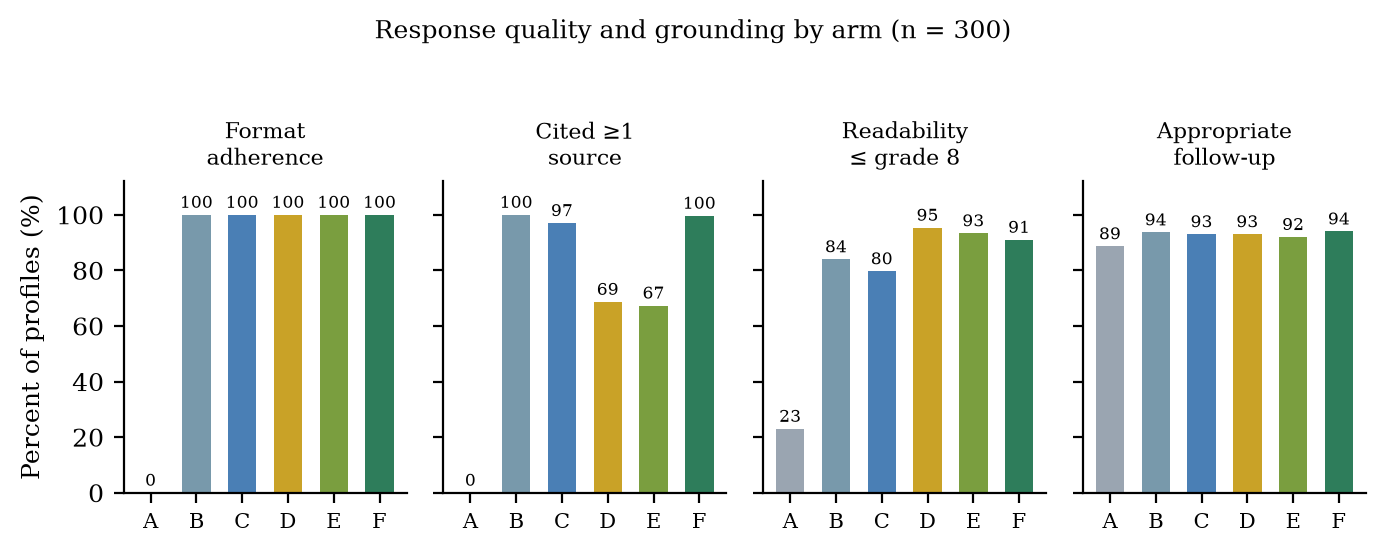
\includegraphics[width=\textwidth]{fig_q1_quality.png}
\caption{Quality and grounding by arm.}
\label{fig:q1quality}
\end{figure}

Three findings stand out.

\textbf{The compact prompt is not viable without fine-tuning.} Arm A---the base
model given the short prompt---achieves 0\% format adherence. The base model
simply does not produce the required five-section structure from a short
instruction. Arm F, the same short prompt with the fine-tuned model, achieves
100\%. This is the clearest evidence in the evaluation that fine-tuning
successfully internalised the output contract, and it justifies the
prompt-compression design.

\textbf{Prompt--model matching drives grounding.} The fine-tuned model under the
\emph{full} prompt (arms D and E) cites a retrieved source in only 68.7\% and
67.3\% of responses, whereas under the \emph{compact} prompt it was trained with
(arm F) that rises to 99.7\%. Because retrieval is identical in all three arms,
this is a prompt--model mismatch effect: applying the fine-tuned model to the
prompt format it was not trained on degrades exactly the behaviour that was
tuned. It is a useful negative result---fine-tuned models should be served with
the prompt they were trained against.

\textbf{Readability improved with fine-tuning.} Readability is scored on the five
patient-facing sections only; the internal grounding line of source
identifiers is excluded because the patient never sees it. Mean Flesch--Kincaid
grade fell from 7.52 (arm B) to 7.16 (arm D) under the same prompt, and the
proportion of responses at or below grade 8 rose from 84.0\% to 95.3\% (paired
difference $+11.3$ points, Holm-significant). The deployed configuration
(arm F) reaches 91.0\% at a mean grade of 7.31; its difference from arm E
(93.3\%) is not significant, so prompt compression carries no measurable
readability cost. The validator slightly lowers readability (C vs B:
$-4.3$ points, Holm-significant): the referral notices and fallback templates it
inserts read at a higher grade level than the model's own prose. Arm A's 23\% is not meaningful, since its output is
structurally malformed.

Retrieval quality was measured on the shared retrieval configuration used by
arms B--F: Recall@4 of 0.806 (the fraction of each profile's expected evidence
topics covered by at least one of the four retrieved passages), Precision@4 of
0.766, MRR of 0.919 and nDCG@4 of 0.917. Every cited source identifier was
valid (rate 1.000), confirming that the deterministic citation layer prevents
invented references. Relevance here is judged by knowledge-base topic matching
as a proxy; no human relevance labelling was performed.

\section{Efficiency}
\label{sec:q1_efficiency}

Table~\ref{tab:q1_eff} and Figure~\ref{fig:q1eff} report token cost and latency.

\begin{table}[H]
\centering
\caption{Mean token usage and latency per request.}
\label{tab:q1_eff}
\begin{tabular}{@{}cl rrrr@{}}
\toprule
\textbf{Arm} & \textbf{Name} & \textbf{Prompt} & \textbf{Completion} &
\textbf{Total} & \textbf{Latency (s)} \\
\midrule
A & base\_compact & 878.8 & 365.7 & 1244.6 & 12.32 \\
B & base\_rag & 2404.0 & 454.3 & 2858.3 & 21.98 \\
C & base\_rag\_val & 2404.0 & 454.3 & 2858.3 & 21.98 \\
D & ft\_rag & 2404.0 & 404.2 & 2808.2 & 28.52 \\
E & ft\_rag\_val & 2404.0 & 404.2 & 2808.2 & 28.52 \\
\textbf{F} & \textbf{ft\_compact\_val} & \textbf{1799.0} & 431.1 &
\textbf{2230.1} & 30.86 \\
\bottomrule
\end{tabular}
\end{table}

\begin{figure}[H]
\centering
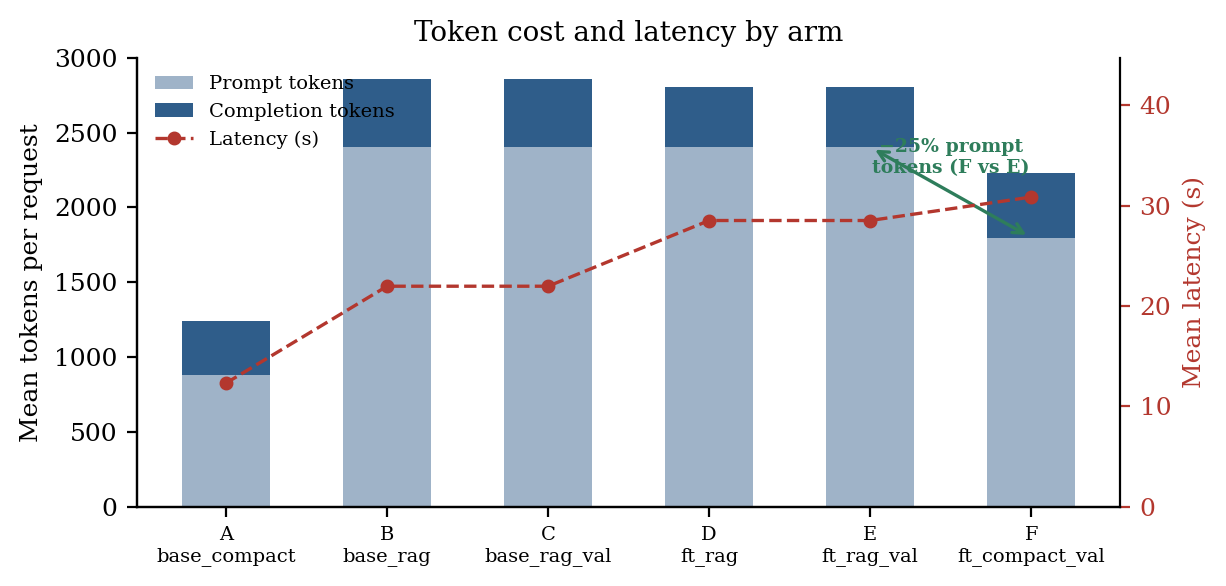
\includegraphics[width=0.92\textwidth]{fig_q1_efficiency.png}
\caption{Token cost and latency by arm. The deployed configuration reduces
prompt tokens by 25\% relative to the full-prompt fine-tuned arm.}
\label{fig:q1eff}
\end{figure}

The deployed configuration uses 1{,}799 prompt tokens against 2{,}404 for the
full-prompt fine-tuned arm, a reduction of 25.2\%, and 22\% fewer total tokens.
This is the direct, measured payoff of the prompt-compression objective.

Latency does not follow token count: arm F is the slowest at 30.9 s despite
having the smallest prompt. This is because the LoRA adapter adds a
per-token computation overhead on the local serving hardware, and because
latency was measured on a shared development machine without batching or
serving optimisation. The token reduction is the robust efficiency result; the
latency figures should be treated as indicative of this hardware only and are
not the basis of any claim.

\section{Unsafe-Category Breakdown}
\label{sec:q1_categories}

Table~\ref{tab:q1_cats} decomposes the delivered violations by category for
selected arms.

\begin{table}[H]
\centering
\caption{Selected delivered violation categories (\% of 300 profiles;
missed red flag is over the 60 emergency profiles).}
\label{tab:q1_cats}
\footnotesize
\setlength{\tabcolsep}{4pt}
\begin{tabular}{@{}c L{1.0in} C{0.78in} C{0.78in} C{0.78in} C{0.85in}@{}}
\toprule
\textbf{Arm} & \textbf{Name} & \textbf{Missed red flag} &
\textbf{False reassur.} & \textbf{Inappr.\ referral} &
\textbf{Severity-wtd harm} \\
\midrule
A & base\_compact & 35.00 & 0.00 & 11.33 & 0.257 \\
B & base\_rag & 25.00 & 0.00 & 6.33 & 0.293 \\
C & base\_rag\_val & \textbf{0.00} & 0.00 & 7.00 & \textbf{0.000} \\
D & ft\_rag & 35.00 & 1.33 & 7.00 & 0.247 \\
E & ft\_rag\_val & \textbf{0.00} & 1.33 & 8.00 & 0.027 \\
\textbf{F} & \textbf{ft\_compact\_val} & \textbf{0.00} & \textbf{0.00} &
6.00 & \textbf{0.000} \\
\bottomrule
\end{tabular}
\end{table}

The deployed configuration is clean on every tracked category, with a
severity-weighted harm score of exactly zero. Arm E retains a small residual
false-reassurance rate of 1.33\%, which the validator does not detect because it
has no corresponding rule---false reassurance is a Q1-only measurement category.
That this pattern appears in E but not in F is consistent with the
prompt-matching effect described in Section~\ref{sec:q1_quality}.

The inappropriate-referral rate---advising urgent care for a profile without
red flags---sits between 6\% and 8\% in the validated arms. This is the cost
side of a sensitivity-first design: the same conservatism that produces 100\%
emergency recall also produces some over-referral. Given that the intervention
being over-recommended is a clinical consultation, this trade is judged
acceptable, but it is a real cost and is reported as such.

\section{Corrections and Audit Trail}
\label{sec:corrections}

Three classes of correction were made during evaluation and are documented here
in full, because the credibility of a safety result depends on the transparency
of the process that produced it.

\textbf{A harness defect.} In the initial run, the free-text symptom associated
with emergency-subgroup profiles existed only in benchmark metadata and was
never inserted into the prompt or the validator context. Approximately 40
profiles were therefore structurally incapable of triggering a redirect. The
harness was corrected to inject the symptom into both, and the affected arms
were regenerated.

\textbf{A retrieval defect.} As described in Section~\ref{sec:stack}, the index
had been built with a lexical fallback embedder rather than BGE-M3. After
correction, arms B through F were regenerated against the corrected index. Arm A
uses no retrieval and was left untouched; its results are byte-identical across
all runs, which serves as an internal control confirming that nothing else
drifted between runs.

\textbf{Scoring defects.} Ten false-positive patterns were identified in the
detection logic---eight in the evaluation detectors and two in the deployed
validator itself. Representative examples: a correct refusal (``do not drink 6
litres a day---that is too much'') was counted as dangerous fluid advice; a safe
deferral (``your doctor may want to adjust your medicine'') was counted as
medication advice; a laboratory description (``your protein levels are slightly
lower'') was counted as a dietary restriction; and a correct reinforcement
(``your risk is \emph{not} high'') was counted as a risk-category contradiction.
All were negation- or scope-handling errors. Each fix was verified with paired
true-positive and false-positive tests, and both the pre-correction and
post-correction runs were re-scored with the same corrected code so that the
comparison remained fair.

Two of the ten defects were in the production validator, not merely in the
evaluation harness, and were fixed at source. Because the validator is a
post-processing step over stored text, re-applying it required no regeneration
and no additional GPU time; the raw model outputs were verified byte-identical
before and after. Notably, one consequence of the scoring corrections was that
an apparent adversarial-attack success in an earlier run was shown to have been
a false positive throughout: attack success was 0\% in the retrieval-enabled
arms in both the original and corrected scoring.

\section{Summary of Findings}
\label{sec:results_summary}

\begin{enumerate}
  \item The screening cascade recovers 70.9\% accuracy, 66.0\% balanced accuracy
        and 73.7\% high-risk recall from routine inputs alone, with 2 high-to-low
        misclassifications out of 38 high-risk participants.
  \item Across all six arms, 6.3\%--10.3\% of raw language-model outputs contain a
        critical safety violation. No configuration of prompting, retrieval or
        fine-tuning eliminated this.
  \item The deterministic validator reduces the delivered rate to zero in both
        the base and the deployed configuration, and lifts emergency-redirect
        recall to 100\%. These are the only effects that survive multiplicity
        correction, and they do so at $p<0.001$.
  \item Fine-tuning did not produce a statistically established safety
        improvement, but did enable the compact prompt (0\% $\rightarrow$ 100\%
        format adherence), improve grounding to 99.7\%, improve readability, and
        reduce destructive fallbacks ninefold.
  \item Prompt compression reduced prompt tokens by 25\% with no measurable
        safety cost.
\end{enumerate}
